\chapter{Hardware-Specific Deployment Pipelines}\label{ap:boards_pipelines}

This appendix explores the specific deployment pipelines required to adapt and run \gls{AI} models across four distinct hardware architectures: the \nameref{ap:pipelines:rpi5}, the \nameref{ap:pipelines:hailo}, the \nameref{ap:pipelines:aicam}, and the \nameref{ap:pipelines:jetson}.

\todo{explicar que son ejemplos de como se harían o como se han adaptado al proyecto??}

\section{\texorpdfstring{\acrshort{RPi}}{RPi}5 \texorpdfstring{\acrshort{CPU}}{CPU}}\label{ap:pipelines:rpi5}

\begin{table}[H]
    \centering
    \caption{\acrshort{RPi}5 \acrshort{CPU} Deployment Pipeline Phases}
    \label{tab:rpi5_cpu_pipeline}
    \begin{tabular}{p{0.15\textwidth}
                    p{0.25\textwidth}
                    p{0.32\textwidth}
                    p{0.18\textwidth}}
        \toprule
        \textbf{Phase} & \textbf{Objective} & \textbf{Process} & \textbf{Output} \\ 
        \toprule
        
        \textbf{1. Model Optimization} \newline \textit{(Cloud / Server Platform)} & 
        Converting dynamic weights to a static, vectorized graph for \gls{ARM} architecture. & 
        Executing \texttt{export\_to\_onnx} to serialize the PyTorch model (\texttt{best.pt}) into an optimized \texttt{.onnx} graph, embedding the \gls{NMS} logic natively (\texttt{nms=True}). & 
        \gls{CPU}-optimized \texttt{.onnx} model binary. \\ 
        \midrule
        
        & 
        & 
        \textbf{Network Transfer} & 
         \\ 
        \midrule

        \textbf{2. Execution} \newline \textit{(Raspberry Pi 5)} & 
        Real-time inference using host \gls{CPU} parallelization. & 
        The \textit{ONNX Runtime} loads the static graph, parallelizes FP32 operations, and executes the embedded \gls{NMS} layers to filter boxes based on the threshold. & 
        Real-time visual stream displaying detection overlays via \texttt{OpenCV}. \\ 
        \bottomrule
    \end{tabular}
\end{table}

\begin{figure}[H]
    \centering
    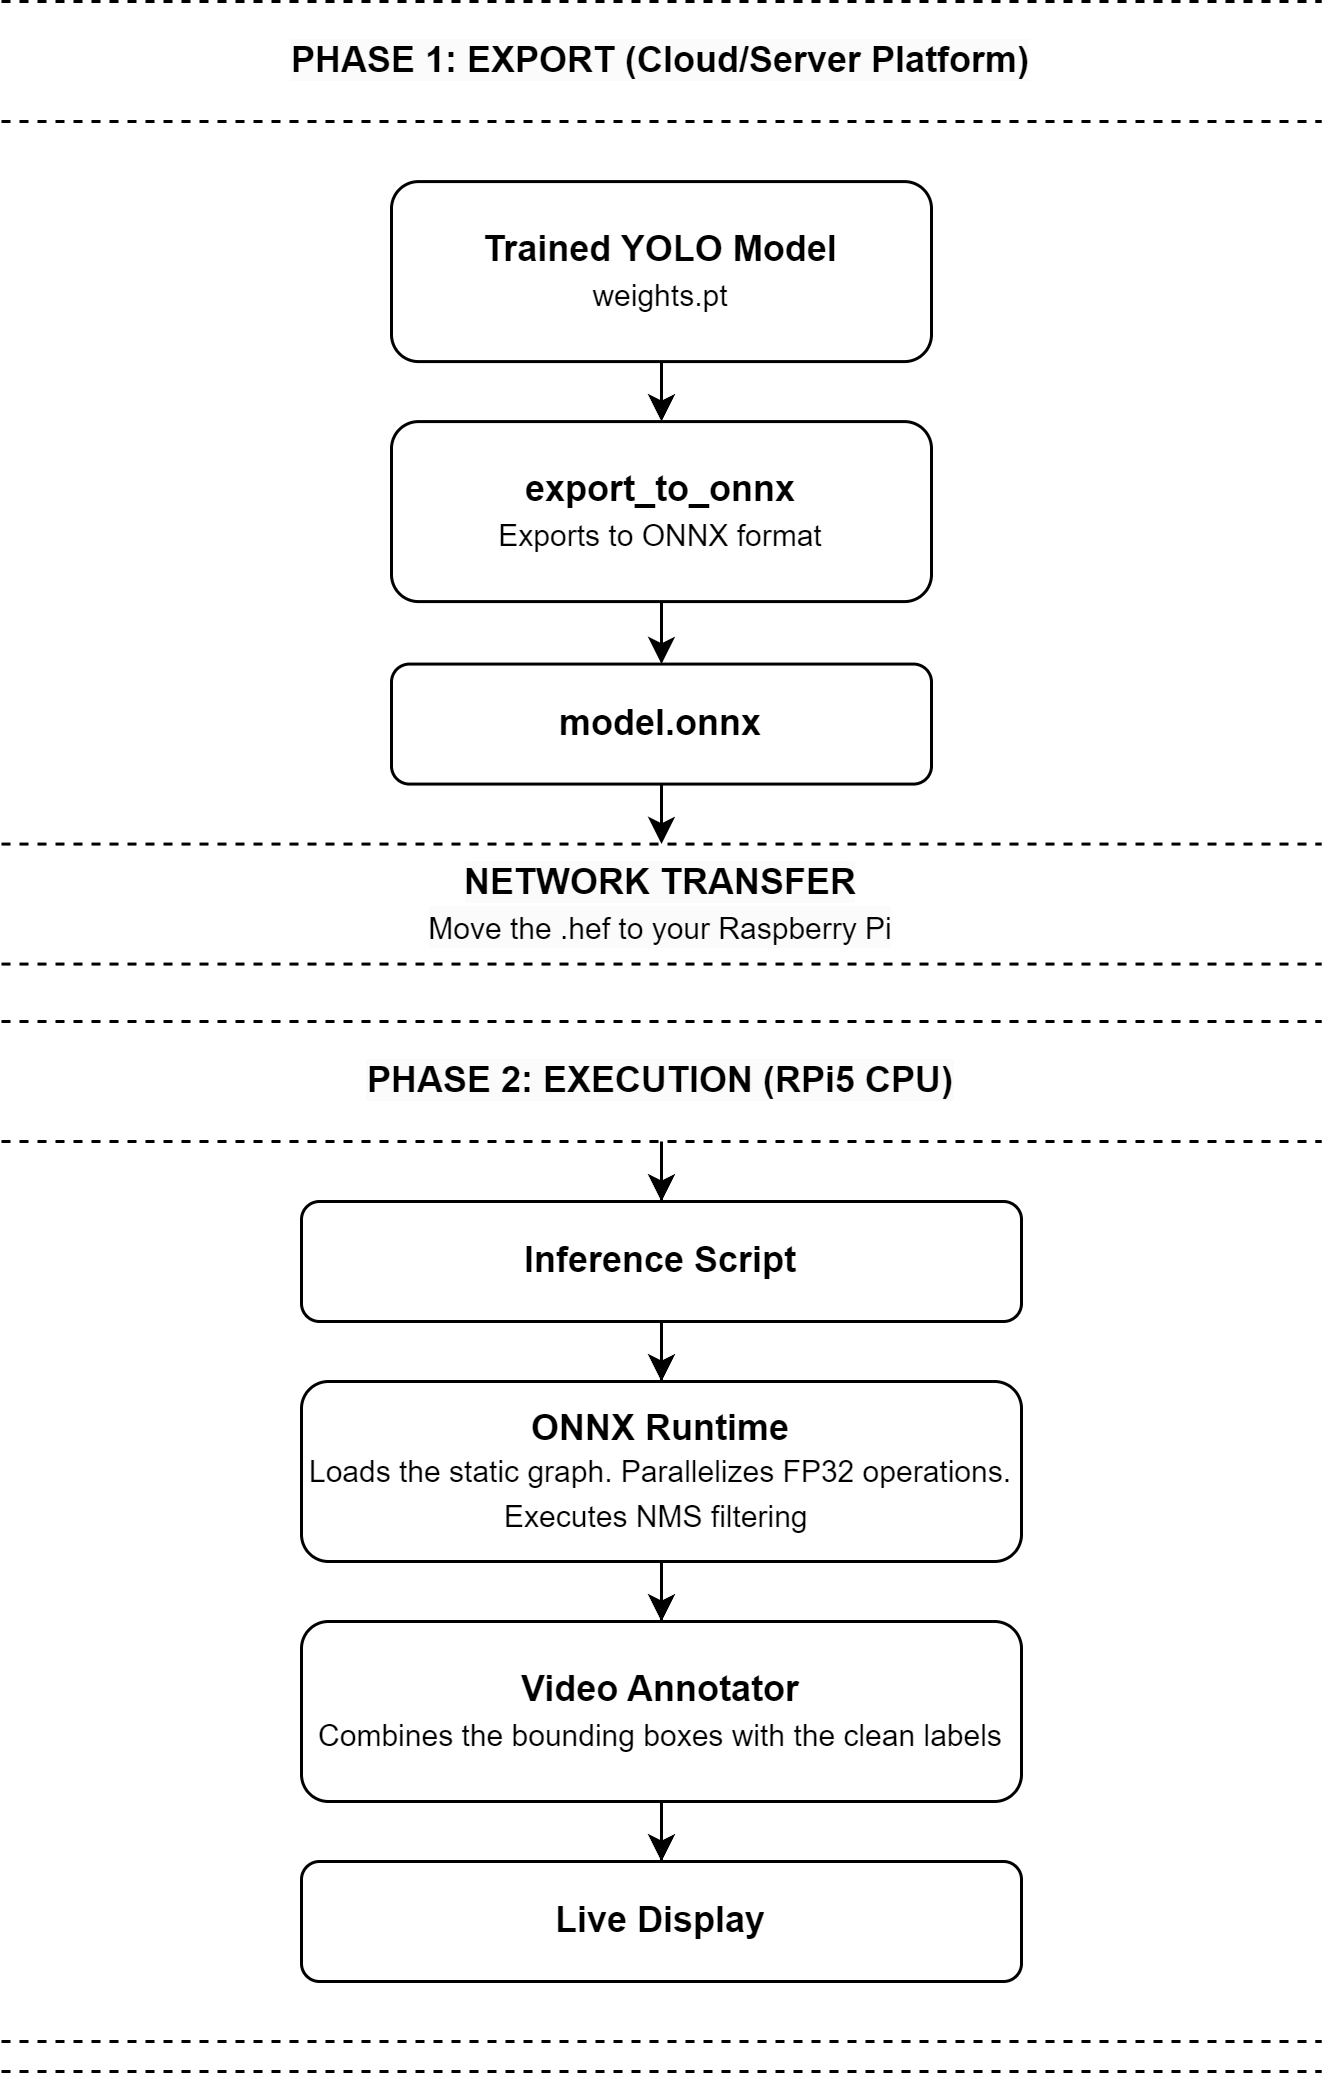
\includegraphics[width=0.8\linewidth]{images/RPi CPU Pipeline.png}
    \caption{\acrshort{RPi}5 \acrshort{CPU} Pipeline}
    \label{fig:rpicpu}
\end{figure}

\clearpage

\section{\texorpdfstring{\acrshort{RPi}}{RPi}5 + Hailo8/8L}\label{ap:pipelines:hailo}

\begin{table}[H]
    \centering
    \caption{Hardware-Specific Deployment Pipeline Phases for Hailo-8/8L}
    \label{tab:hailo_pipeline_phases}
    \renewcommand{\arraystretch}{1.5}
    \rotatebox{90}{
    \begin{tabular}{p{0.23\textwidth}
                    p{0.3\textwidth}
                    p{0.4\textwidth}
                    p{0.28\textwidth}}
        \toprule
        \textbf{Phase} & \textbf{Objective} & \textbf{Process} & \textbf{Output} \\ 
        \toprule
        
        \textbf{1. Preparation} \newline \textit{(Cloud / Server Platform)} & 
        Structuring model graphs and validation assets for \gls{NPU} ingestion format constraints. & 
        Running \texttt{export\_to\_onnx} to convert the PyTorch model (\texttt{best.pt}) while stripping \gls{NMS} layers (\texttt{nms=False}, \texttt{opset=11}). Concurrently running \texttt{hailo\_calibration\_data} to validate, scale, and center-crop exactly 1,024 images. & 
        Optimized intermediate \texttt{<ONNX\_MODEL>.onnx} file and a structured \texttt{calib/} data directory. \\ 
        \midrule
        
        \textbf{2. Compilation} \newline \textit{(Cloud / Server Platform \& Docker)} & 
        Translating abstract mathematical graphs into physical INT8 quantization instruction sets. & 
        Spinning up the isolated \textit{Hailo \gls{AI} SW Suite} Docker container, mounting assets to the \texttt{shared\_with\_docker} workspace, and executing \texttt{hailomz compile} to quantize weights and schedule layouts via network configuration files (\texttt{--hw\_arch hailo8 or hailo8l}). & 
        Compiled standalone Hailo Executable Format (\texttt{.hef}) target binary. \\ 
        \midrule

        & 
        & 
        \textbf{Network Transfer} & 
         \\ 
        \midrule
        
        \textbf{3. Execution} \newline \textit{(Hailo-8 / 8L Edge Device)} & 
        Executing low-latency parallelized matrix math while decoding visual boxes in real time. & 
        Deploying the \gls{NPU} application script. The Hailo \gls{NPU} handles high-\gls{FPS} execution of INT8 neural operations, while the Host \gls{CPU} concurrently intercepting raw output matrices, applies the \gls{NMS} fallback calculations, and triggers the video annotator layers. & 
        Live visual display output rendering real-time streaming media with smooth inference overlays. \\ 
        \bottomrule
    \end{tabular}
    }
\end{table}

\begin{figure}[H]
    \centering
    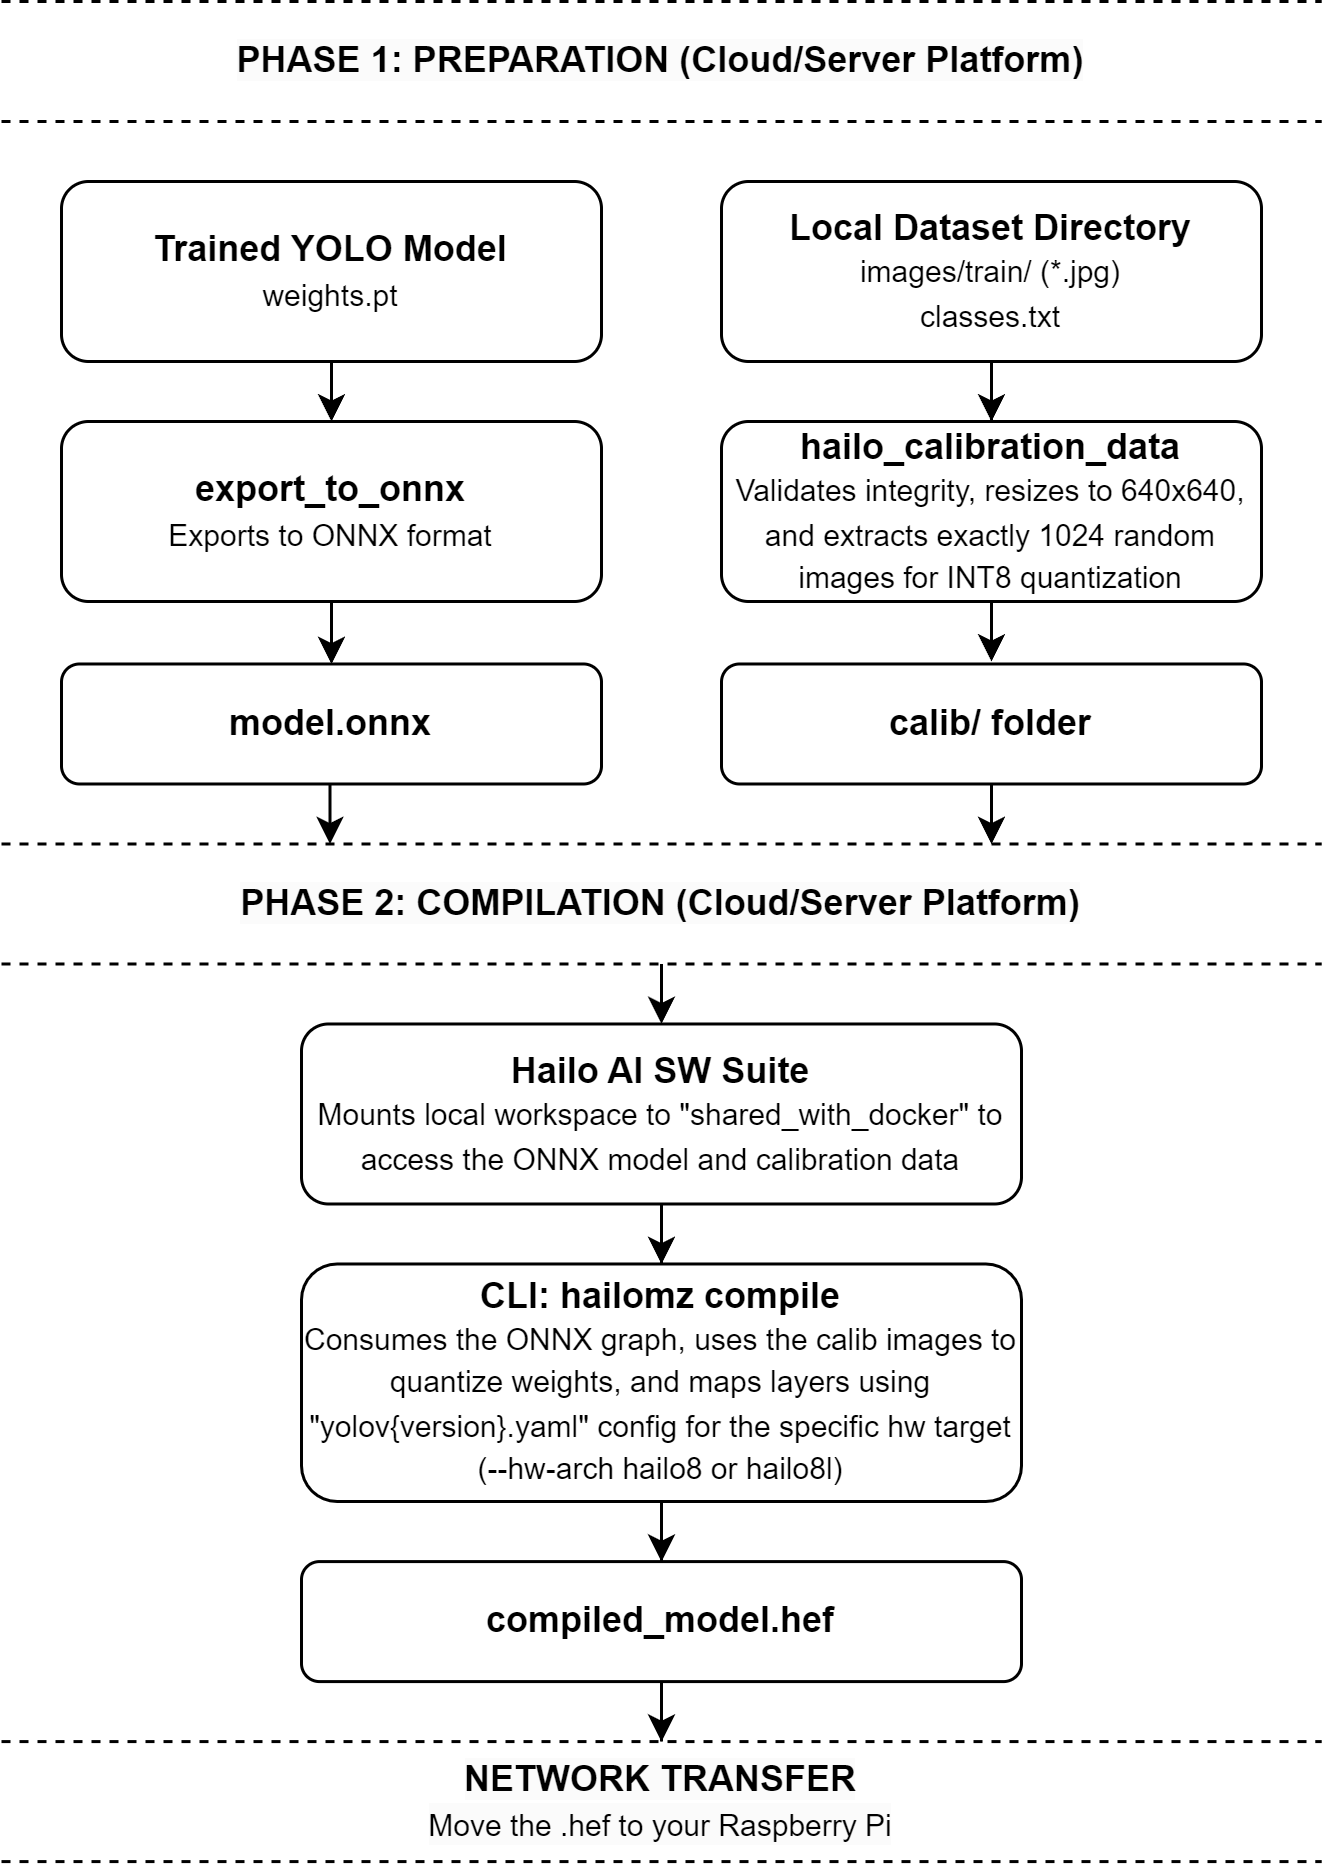
\includegraphics[width=0.8\linewidth]{images/Hailo Pipeline 1.png}
    \caption{\acrshort{RPi}5 + Hailo-8/8L Pipeline (1)}
    \label{fig:hailo_1}
\end{figure}

\begin{figure}[H]
    \centering
    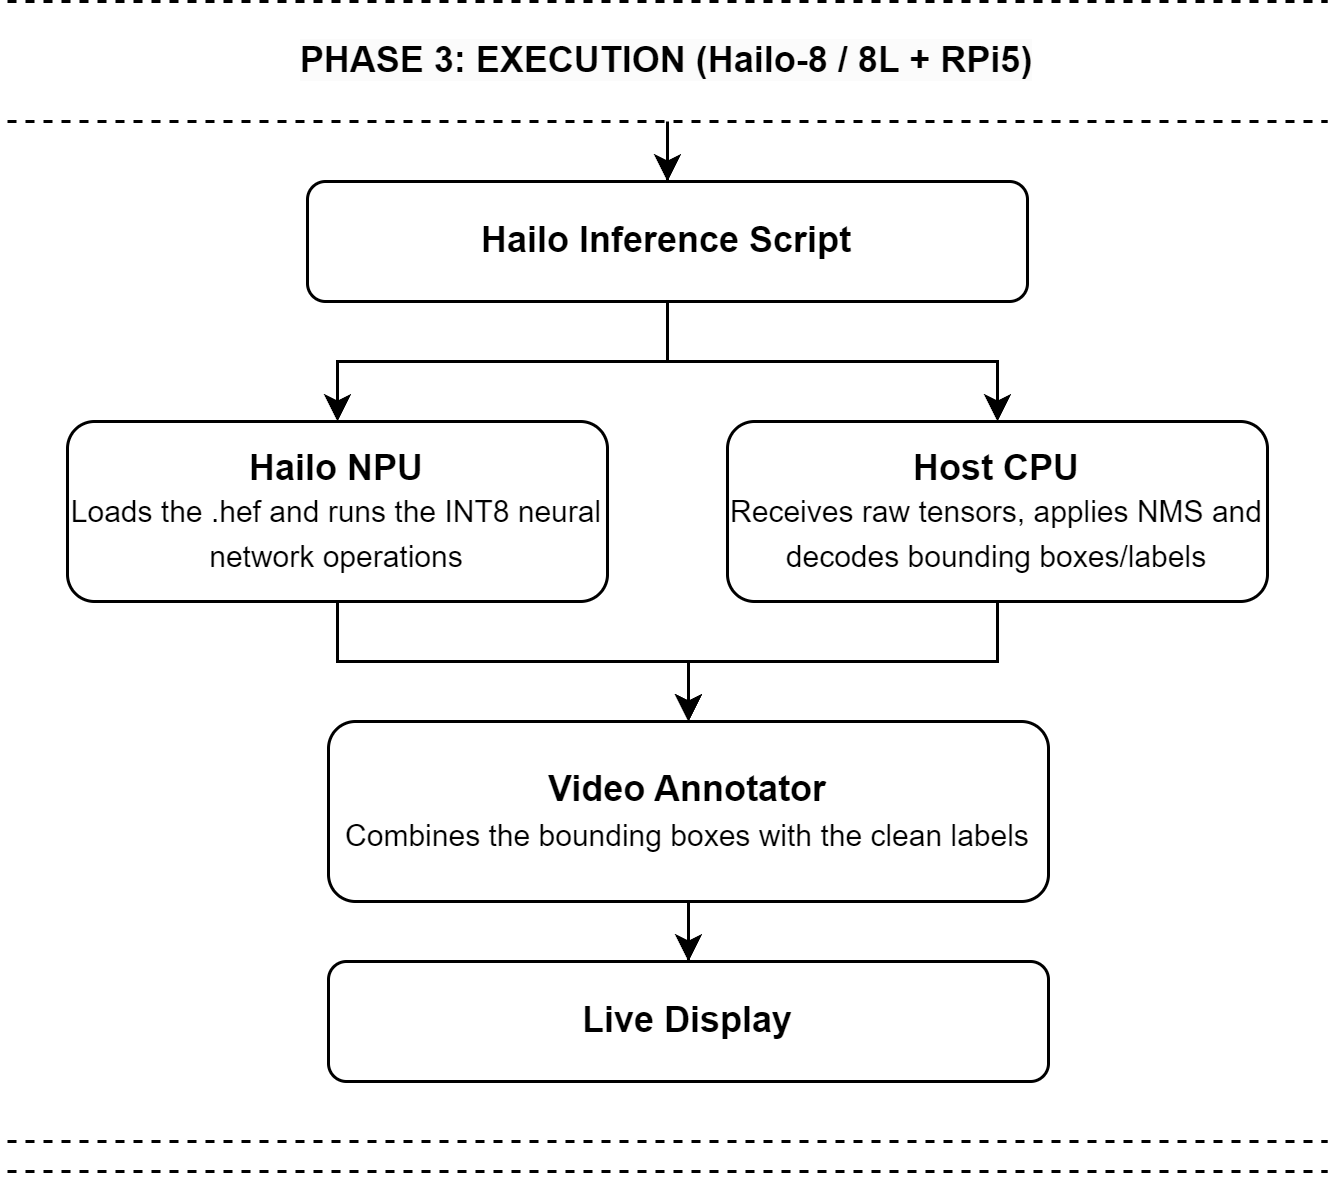
\includegraphics[width=0.8\linewidth]{images/Hailo Pipeline 2.png}
    \caption{\acrshort{RPi}5 + Hailo-8/8L Pipeline (2)}
    \label{fig:hailo_2}
\end{figure}
\clearpage

\clearpage

\section{\texorpdfstring{\acrshort{RPi}}{RPi}5 + \texorpdfstring{\acrshort{RPi}}{RPi}5 \texorpdfstring{\acrshort{AI}}{AI} Camera}\label{ap:pipelines:aicam}

\begin{table}[H]
    \centering
    \caption{Hardware-Specific Deployment Pipeline Phases}
    \label{tab:ai_cam_phases}
    \renewcommand{\arraystretch}{1.5}
    \rotatebox{90}{
    \begin{tabular}{p{0.23\textwidth}
                    p{0.3\textwidth}
                    p{0.4\textwidth}
                    p{0.28\textwidth}}
        \toprule
        \textbf{Phase} & \textbf{Objective} & \textbf{Process} & \textbf{Output} \\ 
        \toprule
        
        \textbf{1. Model \& Data Prep} \newline \textit{(Cloud/Server Platform)} & 
        Adapting the workspace for Sony's tools. & 
        Cleaning the trained model and class names; creating an image path map for network calibration. & 
        Dynamic \texttt{.yaml} config file with absolute paths and clean classes. \\ 
        \midrule
        
        \textbf{2.1 Exportation \& Optimization} \newline \textit{(Cloud/Server) Platform} & 
        Optimizing the model for the camera's limited memory and energy constraints. & 
        Calibrating with real dataset images to flatten the model, reducing heavy 32-bit floating-point weights to lightweight 8-bit integers. & 
        Generic, compressed model (typically \texttt{.onnx} format). \\ 
        \midrule
        
        \textbf{2.2 Compilation for Hardware} \newline \textit{(Cloud/Server) Platform} & 
        Translating the generic model into physical instructions for the Sony IMX500 chip. & 
        The Sony converter distributes processing across the camera's NPU cores and translates the model into hardware-readable binaries. & 
        Compressed \texttt{packerOut.zip} file. \\ 
        \midrule

        & 
        & 
        \textbf{Network Transfer} & 
         \\ 
        \midrule
        
        \textbf{3. Final Packaging} \newline \textit{(\gls{RPi}5)} & 
        Creating a specific container with image ingestion rules for the binaries. & 
        Wrapping the \texttt{.zip} with metadata regarding color format and tensor structure using \gls{RPi} \gls{OS} native tools (\texttt{imx500-tools}). & 
        Final executable \texttt{network.rpk} (\gls{RPi} Package) for camera injection. \\ 
        \midrule
        
        \textbf{4. Execution \& Post-Processing} \newline \textit{(\gls{RPi}5 + \gls{AI} Cam)} & 
        Dividing inference processing between the camera chip and the \gls{RPi}. & 
        The \texttt{.rpk} is flashed into the camera sensor, which processes the neural network. The \gls{RPi} filters the returned raw data matrices and draws bounding boxes. & 
        Real-time video stream displaying smooth inference results. \\ 
        \bottomrule
    \end{tabular}
    }
\end{table}

\begin{figure}[H]
    \centering
    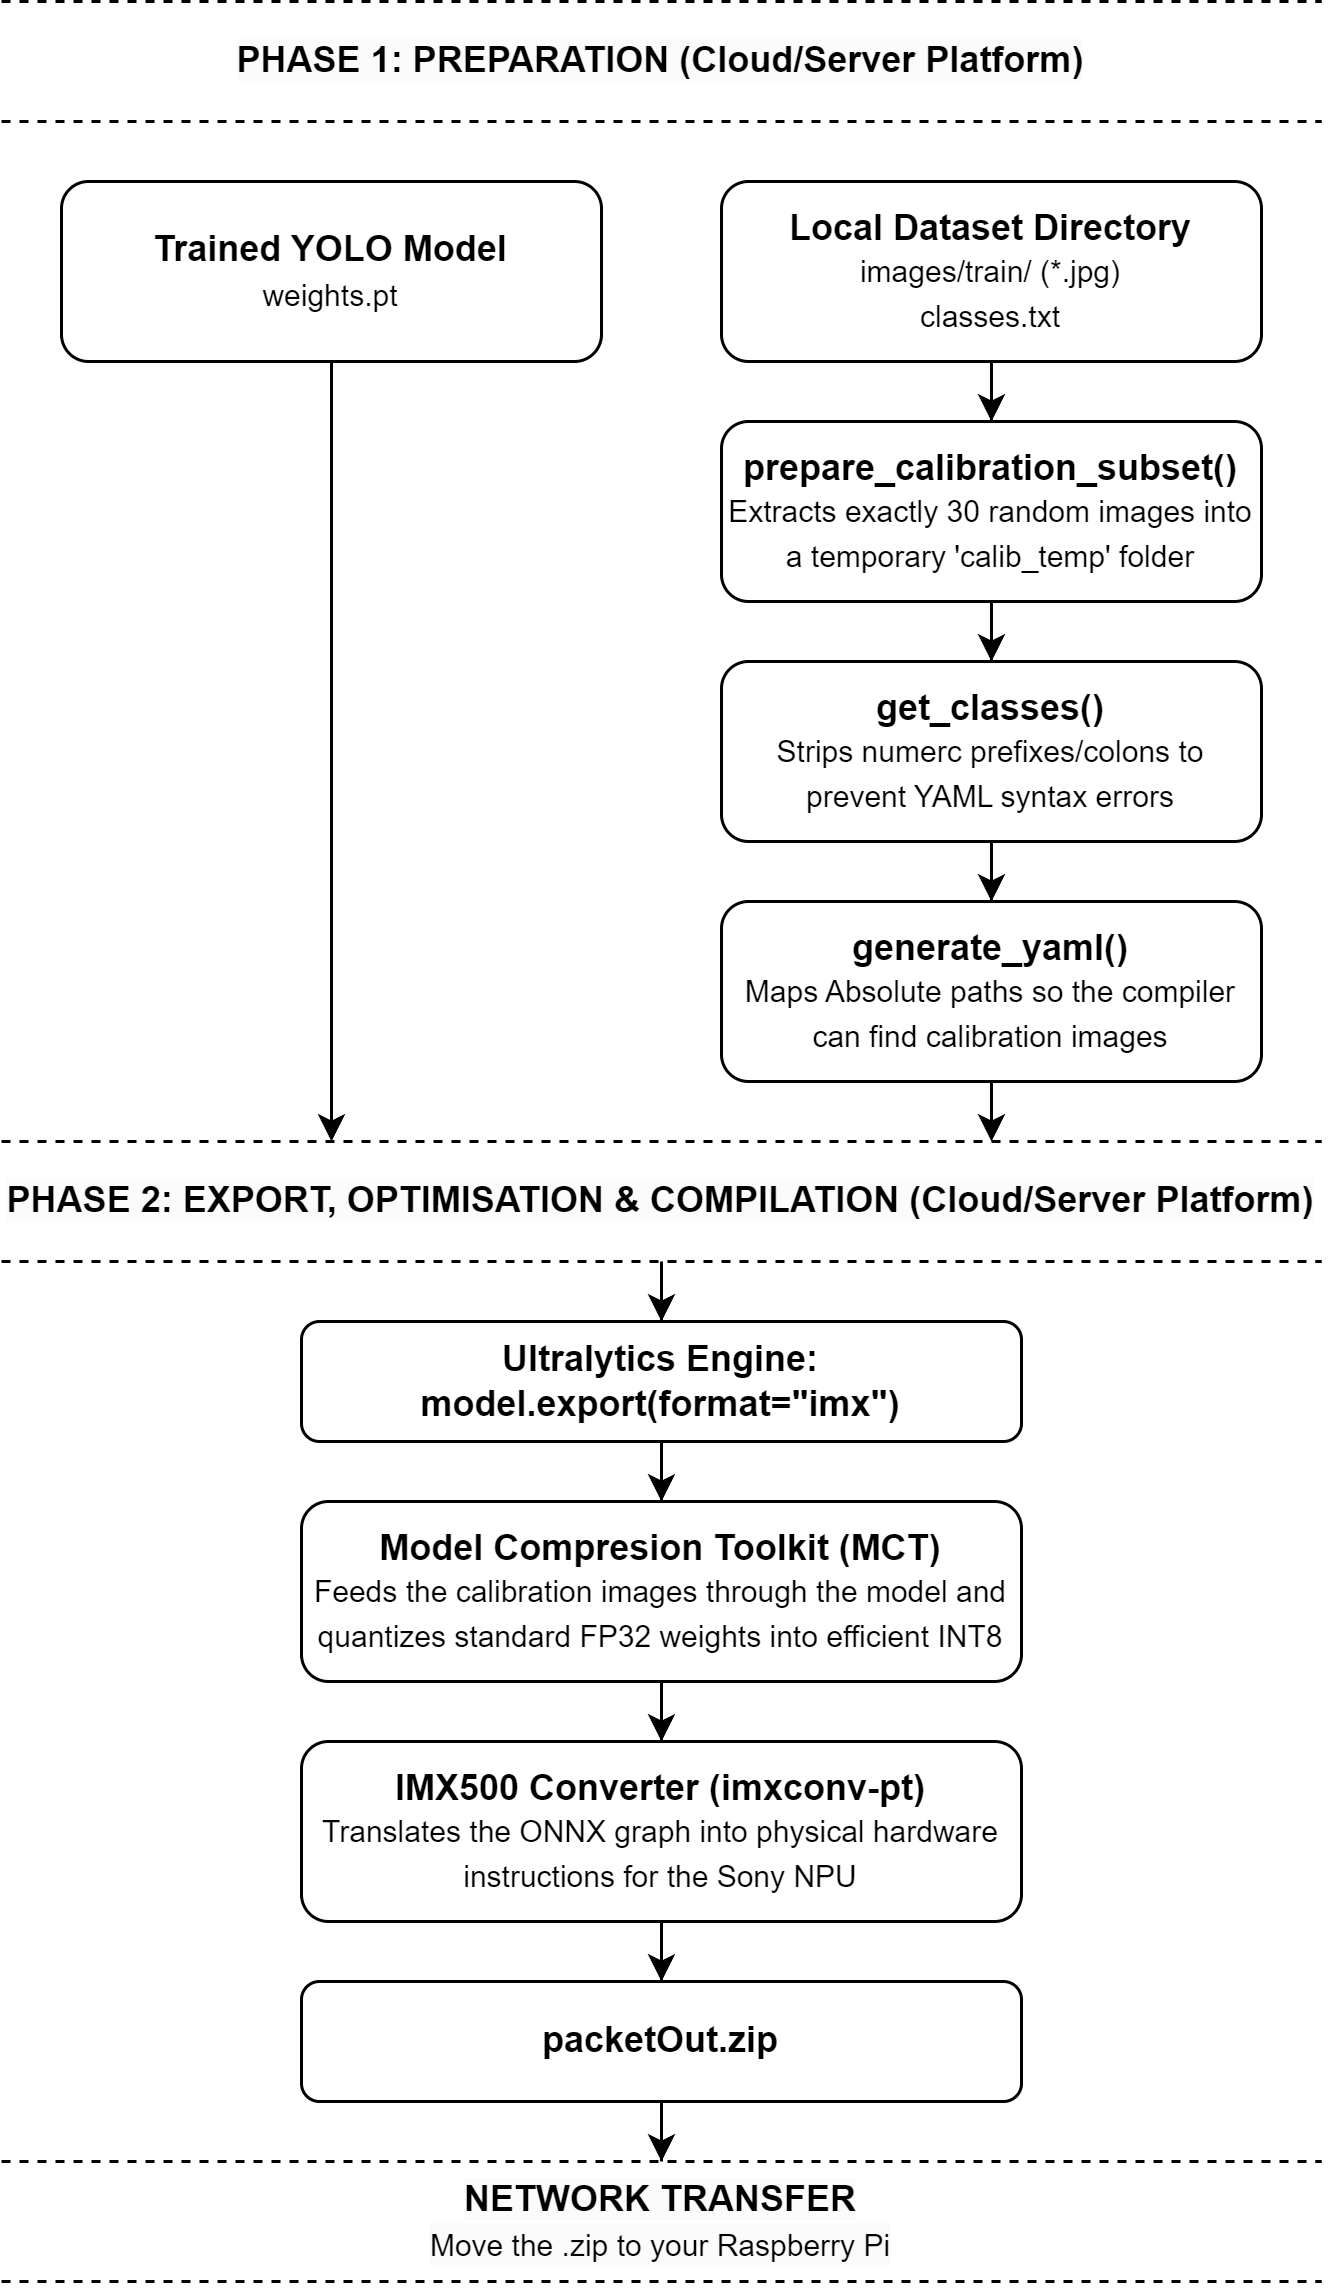
\includegraphics[width=0.8\linewidth]{images/AI Cam Pipeline 1.png}
    \caption{\acrshort{RPi}5 + \acrshort{RPi}5 \acrshort{AI} Camera Pipeline (1)}
    \label{fig:ai_cam_1}
\end{figure}

\begin{figure}[H]
    \centering
    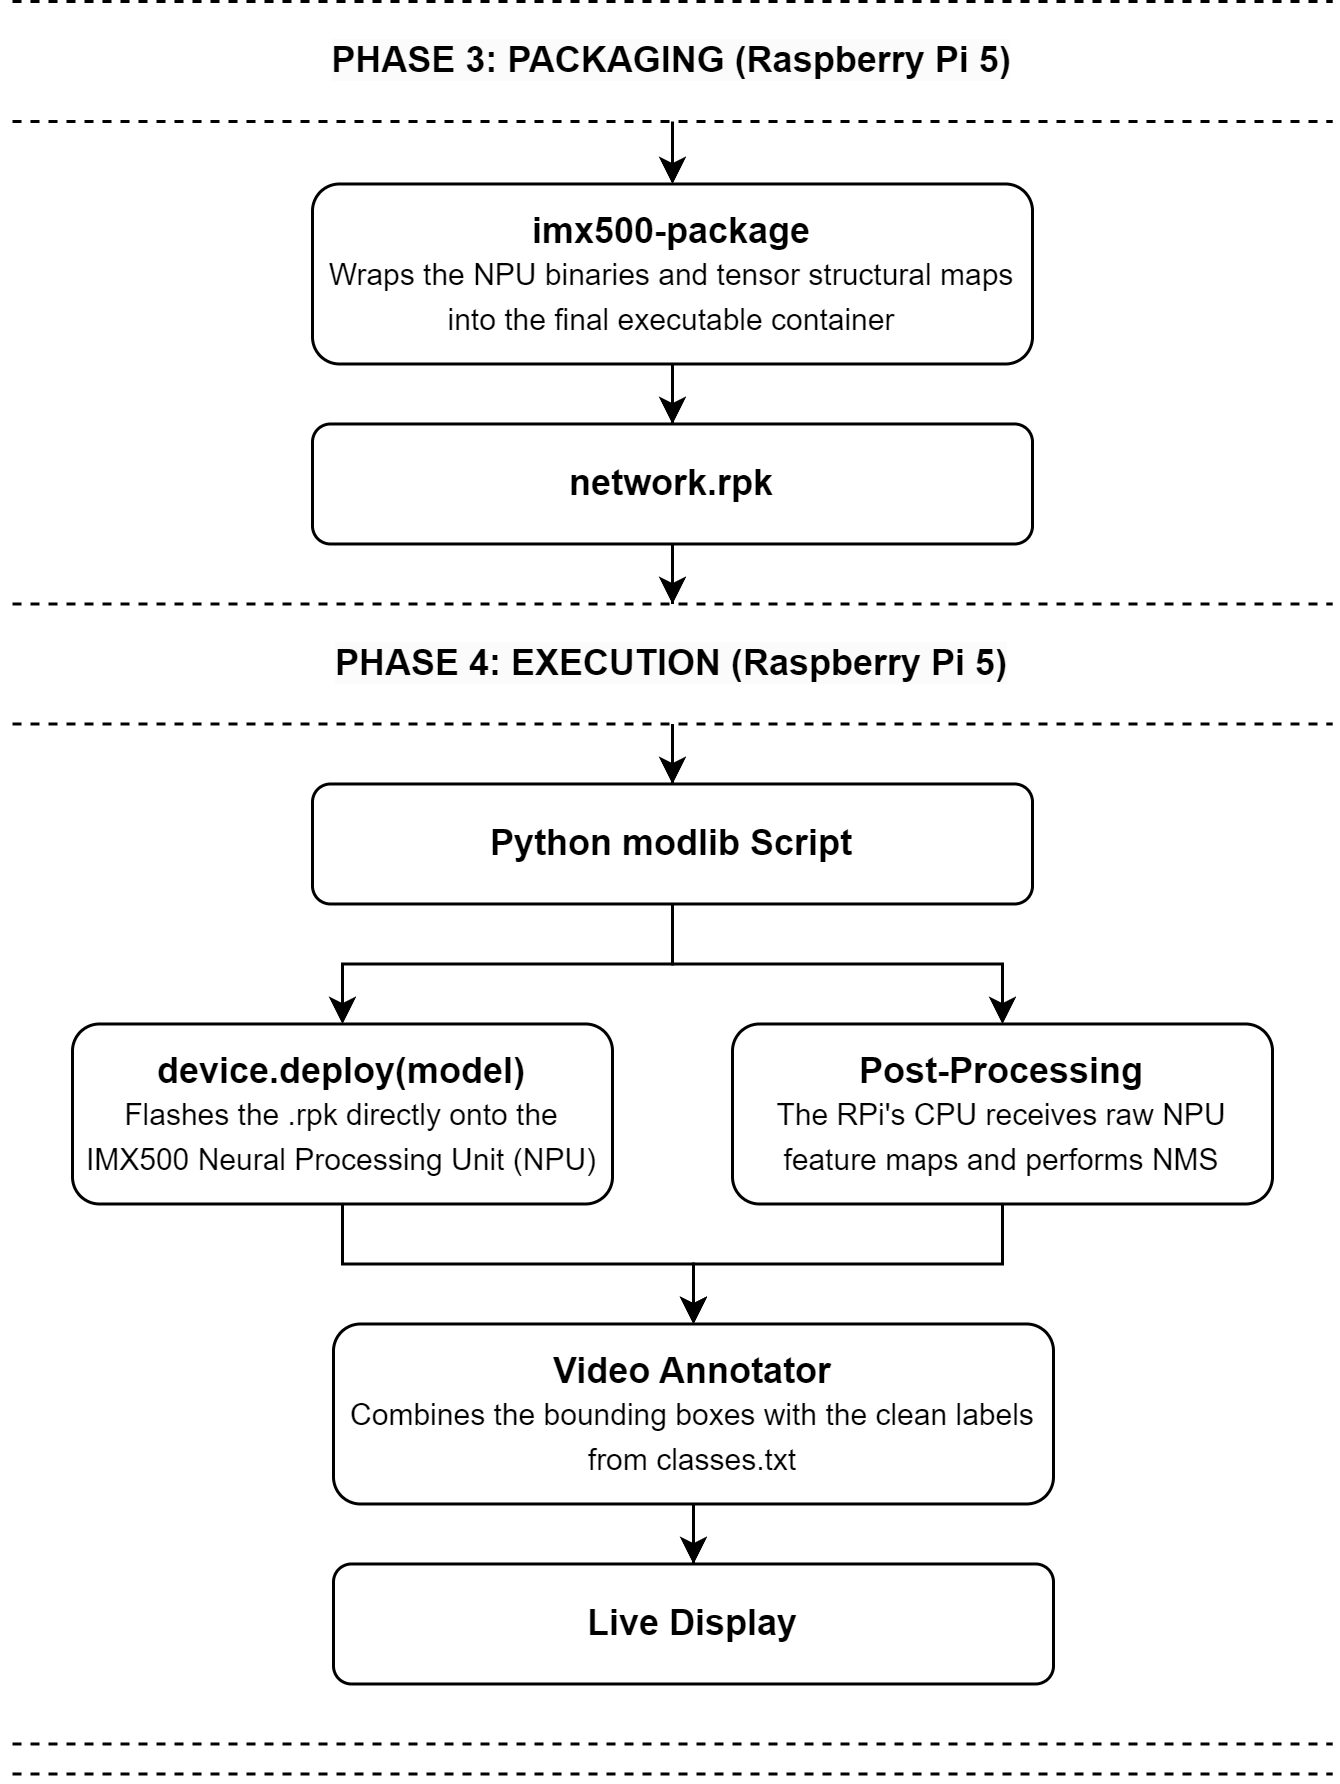
\includegraphics[width=0.8\linewidth]{images/AI Cam Pipeline 2.png}
    \caption{\acrshort{RPi}5 + \acrshort{RPi}5 \acrshort{AI} Camera Pipeline (2)}
    \label{fig:ai_cam_2}
\end{figure}
\clearpage

\section{NVIDIA Jetson Orin Nano}\label{ap:pipelines:jetson}

\todo{jetson pipeline} 